\documentclass[twosided,a4,10pt]{article}
\usepackage[utf8]{inputenc}
\usepackage{amsmath}
\usepackage{amsfonts}
\usepackage{amssymb}
\usepackage{textcomp}
\usepackage{graphicx}
\usepackage[usenames,dvipsnames]{xcolor}
\usepackage{pifont}
\usepackage{nicefrac}
\usepackage{sectsty}
\usepackage{lipsum}  
\usepackage{setspace}

% ------
% Fonts and typesetting settings
\usepackage[sc]{mathpazo}
\usepackage[T1]{fontenc}
\linespread{1.1} % Palatino needs more space between lines
\usepackage{microtype}
\subsectionfont{\fontsize{10}{15}\selectfont}

% ------
% Page layout
\usepackage[hmarginratio=1:1,top=32mm,columnsep=20pt]{geometry}
\usepackage[font=it]{caption}
\usepackage{paralist}
\usepackage{multicol}

% ------
% Abstract
\usepackage{abstract}
	\renewcommand{\abstractnamefont}{\normalfont\bfseries}
	\renewcommand{\abstracttextfont}{\normalfont\small\itshape}


% ------
% Titling (section/subsection)
\usepackage{titlesec}
\renewcommand\thesection{\Roman{section}}
\titleformat{\section}[block]{\large\scshape\centering}{\thesection.}{1em}{}

% ------
% Clickable URLs (optional)
\usepackage{hyperref}

% ------
% Header/footer
\usepackage{fancyhdr}
	\pagestyle{fancy}
%	\fancyhead{}
	\fancyfoot[C]{Wissenschaftliches Seminar WS 2017/18 $\cdot$
          Software Engineering $\cdot$ Prof. Skornia}
	\fancyhead[C]{OTH Regensburg $\cdot$ Fakultät IM \newline \newline } 
	\fancyfoot[RO,LE]{\thepage}



% ------
% Maketitle metadata
\title{\vspace{-5mm}%
	\fontsize{20pt}{10pt}\selectfont
	\textbf{Adventures in Attacking Wind Farm}
	}	
\vspace{-5mm}\date{}
\author{
	\large
       \begin{minipage}[t]{0.33\linewidth}
         \begin{center}
           	\textsc{Butrint Dehari}\\[2mm]
                 \normalsize	Matr.nr: 3118661\\
                 \normalsize
                 \href{mailto:autor1@stud.oth-regensburg.de}
                 {butrint.dehari@st.oth-regensburg.de}      
         \end{center}
       \end{minipage}        
       \begin{minipage}[t]{0.33\linewidth}
         \begin{center}
           	\textsc{Celestin Mouangue}\\[2mm]
                 \normalsize	Matr.nr: 3080216\\
                 \normalsize
                 \href{mailto:autor2@stud.oth-regensburg.de}
                 {celestin.mouangue@st.oth-regensburg.de}      
         \end{center}
       \end{minipage}
       \begin{minipage}[t]{0.33\linewidth}
         \begin{center}
           	\textsc{Zhong XU}\\[2mm]
                 \normalsize	Matr.nr: 3148136\\
                 \normalsize
                 \href{mailto:autor3@stud.oth-regensburg.de}
                 {zhong.xu@st.oth-regensburg.de}      
         \end{center}
       \end{minipage}
     }





\begin{document}

\maketitle
\thispagestyle{fancy}

\begin{abstract}
\noindent 
Because of global warming issues, many countries around the world have began to adopt wind farm energy. Being a new emerging technology it still lacks the experience in the security field and therefor it has become a target of attacks. Attackers can easily access and damage the windfarm. In this paper we explain what a wind farm is, what protocols are used to communicate with the wind farm, what types of security breaches can be done and how to prevent these attacks.
\end{abstract}
\begin{multicols}{2}


\section{Chapter 1 : General Introduction}
 \subsection{Why Wind Energy?}
 \subsubsection{Climate Change}
 Today we are threatened by global warming and climate change and therefore the energy industry should try to find energy sources free of carbon dioxide pollution and one of the options is generating electricity from wind energy. Wind and solar energy produce only 4\% of the global supply of electricity while coal, the worst fossil fuel polluter, is still the main energy source for generating electricity. So, producing electricity from wind is where we should be working towards in order to avoid any other environmentally unfriendly material for producing electricity. Hopefully with mass production and bigger and more efficient wind turbines, wind energy and other renewable forms of energy will become cheaper and more convenient to use than fossil fuel and therefore become the main source of producing energy.
 \subsubsection{Advantages of Wind Energy}
 Using wind turbines for electricity generation has many advantages and they have been the main reason for their rapid development.
 \begin{description}
 	\item[$\bullet$]
 	 \textit{Provision for a clean source of energy.} Wind energy delivers electricity without producing carbon dioxide. The relatively small amount of GHG (Green House Gas) emissions is produced in the manufacture and transport of the turbines and blades.
 	\item[$\bullet$] \textit{Sustainability.} Energy is sent to the grid whenever the sun shines and the wind blows and this makes wind a sustainable source of energy and another reason to invest in wind farms.
 	\item[$\bullet$] \textit{Location.} Wind turbines can be erected almost anywhere and often they are not in competition with urban development or other land usage.
 	\item[$\bullet$]
 	\textit{Stability of cost of electricity.} Once the wind farm is in place the cost of electricity to customers should be stable.
 	\item[$\bullet$]
 	\textit{Cost effectiveness.} Due to mass production and improved design, the cost of producing electricity from wind has significantly decreased.
 	\item[$\bullet$]
 	\textit{Creation of jobs and local resources.} Thousands of workers are employed for the different processes like the manufacture process, transport of turbines or erection of turbines. Wind Energy projects can be of great help in developing local resources, labor, capital, and even materials.
 \end{description}
 
 \subsubsection{Challenges facing the Wind Energy} Making use of the power of the wind comes with some challenges.
 \begin{description}
 	\item[$\bullet$]
 	\textit{Sporadicity of wind.} The most important problem with producing electricity from wind is that wind is unpredictable. It may not be blowing when the electricity from the wind farm is needed.  
 	\item[$\bullet$]
 	\textit{Good sites are often in remote locations.} This means that the electricity produced onshore has to be transported from these remote locations along expensive high-voltage cable to reach the customers.
 	\item[$\bullet$]
 	\textit{Noise pollution.} The noise coming from the rotating wind turbine falls exponentially with distance from the tower, and at 500 m the sound level is less than 35 dB which is not very much when normal conversation is rated at 60 dB.
 	\item[$\bullet$]
 	\textit{Turbine blades can damage wildlife.} The turning blades of wind turbines are the cause of more than 33, 000 bird deaths in the United States.
 	\item[$\bullet$]
 	\textit{Safety.} One of the main reasons that wind turbines are erected away from human habitation is because of safety issues. If a blade would come adrift it would cause serious harm to people or animals nearby.
 	\item[$\bullet$]
 	\textit{New and unfamiliar technology.} Most of the general engineers are unfamiliar with the wind turbines and therefore when installing new wind turbines in some rural areas, it is a good practice to have some trained staff around the area, in case of a malfunction.
 	\item[$\bullet$]
 	\textit{Initial cost.} This is the most serious drawback of setting up a new wind farm and also the main reason why many governments offer subsidies.
 	
 \end{description}

\subsection{Anatomy of a Wind Turbine}
 \subsubsection{Rotors and Blades}
 %Und noch etwas Text... \cite{muster} \newline
 The rotor is the element that captures energy from the wind. The efficiency depends on the number of the blades in the rotor, their shape, their length and the speed at which the rotor turns. The tip speed ratio determines the speed at which a wind turbine rotor turns. It should be an optimum so that each blade should pass through the air and the turbulence it creates should have dissipated before the next blade arrives in the same position.

\subsubsection{The Drive Train, Nacelles and Towers}
\begin{description}
\item[$\bullet$] 
The drive train connects the energy capturing rotor of a wind turbine to the generator which produces the unit's electrical power. The drive train is composed of the gearbox and the generator. The gearbox is responsible for connecting the low-speed shaft attached to the turbine blades to the high-speed shaft attached to the generator. The gearbox converts the slow rotation of the outer blades, typically 30-60 rpm (Rotation per minute), to the roughly 1000-1800 rpm that the generator needs to start producing energy.
\item[$\bullet$] 
The house of all the main components of the machine except the rotor is called a nacelle. The components include the drive shaft, a gearbox, the generator, a brake to stop the turbine rotating in very low or very high winds and a range of hydraulics and servo systems that control the blade pitch, the rotor speed and the orientation of the complete nacelle structure. Nacelles are usually equipped with a helicopter pad to make it easier for the maintenance crew to land on top of the nacelle. This is very useful on offshore where the maintenance can be difficult sometimes. 
\item[$\bullet$] 
The tower's purpose is to raise the rotor so that it's blades are clear off the ground and of any other obstacle. The higher the turbine rotor is mounted, the stronger the wind, so it is better to raise the nacelle on the highest tower possible. Usually a tower's height is two or three times the blade length. There are different types of towers including: tubular steel towers, lattice towers or concrete towers.

\end{description}

\section{Chapter 2 : Wind Farm Infrastructure }
 \subsection{Wind farm communication infrastructure}
  \subsubsection{Overview of IEC-61400-25 standard}
  	The IEC-61400-25 standard was developed because different Wind Power Plant(WPP) technologies from different manufacturers resulted in technical, implementation and maintenance difficulties. The focus of this standard is on the communication between power plant components like wind turbines and actors like SCADA systems. A SCADA (Supervisory control and data acquisition) system is a software system that is used for controlling, monitoring and analyzing a process. This software communicates with the controller that is running the actual process. Typically these controllers would be PLC(Programmable Logic Controllers) or RTU(Remote Control Unit). The SCADA system gathers real time information from these controllers and brings them to the system where they are presented in a Graphical User Interface to the operators that are running the process.\newline
  	IEC 61400-25 defines a communication model for monitoring and controlling of wind power plants, and this model is comprised of three parts:
  	\begin{enumerate}
  		\item Wind power-plant information model
  		\item Information exchange model
  		\item Mapping the wind power-plant information model and the information exchange model to standard communication profiles. For mapping to web services the information exchange between SCADA systems and wind power-plants is done with SOAP messages.
  	\end{enumerate}	
  	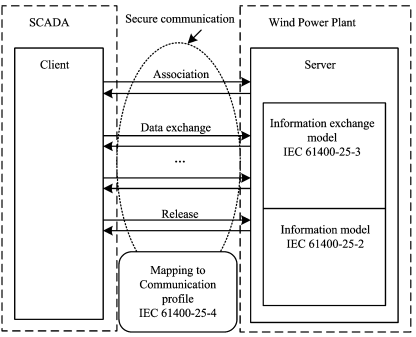
\includegraphics[scale=0.65]{IECProtocol.png}
  	\textit{Fig.1 Communication model for wind power plants defined in IEC 61400-25.} \newline
  	\subsubsection{Security requirements}
  	The information exchange model provides services that are grouped as operational functions and management functions. The security requirements of these two functions include:
  	\begin{enumerate}
  		\item \textit{authentication}: determining the identity of the user;
  		\item \textit{authorization}: ensure that the entity has the correct access;
  		\item \textit{integrity}: messages are protected against unauthorized modification;
  		\item \textit{confidentiality}: objects of the wind power-plant information model are protected and only disclosed to the right users;
  		\item \textit{non repudiation}: preventing a user involved in a data exchange from denying that it participated in the exchange;
  		\item \textit{prevention of denial of service}: preventing a client/server from blocking access to authorized users.
  	\end{enumerate}	
  	In Fig.1 we can see that the communication process of wind power plants can be broken in three steps:
  	\begin{enumerate}
  		\item \textit{associate};
  		\item \textit{data exchange};
  		\item \textit{release}.
  	\end{enumerate}
  	Each of these steps has different security requirements, as listed in Fig.2.	
  	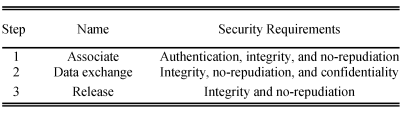
\includegraphics[scale=0.65]{securityRequirements.png}
  	\textit{Fig.2 Security requirements of different communication steps.} \newline	
  	\subsubsection{SOAP web services and security}
  	 Web services are software applications which can be described, located, published and invoked over the network. They are loosely coupled because the client invoking the web service doesn't have to know about the implementation details of the service itself, it just has to know the available methods which can be called on the service and the format which it can understand. SOAP web services are comprised of several technologies and protocols in order to be able to transform and transport the data from a client to a web service in a standard way. Some of the most important ones are the following:
  	\begin{description}
  		\item[$\bullet$] 
  		UDDI(Universal Description, Discovery and Integration): it is used for storing and categorizing web service interfaces.
  		\item[$\bullet$]
  		WSDL(Web Service Description Language): defines the interface, data and message types, interactions and protocols.
  		\item[$\bullet$]
  		SOAP(Simple Object Access Protocol): it is an XML-based messaging protocol for exchanging information.
  		\item[$\bullet$]
  		HTTP(Hypertext Transfer Protocol): messages between the different parts involved are exchanged using the HTTP transport protocol.
  		\item[$\bullet$]
  		XML(Extensible Markup Language): is the basic foundation on which web services are built and defined.
  	\end{description} 	
  	WS security is an extension to SOAP to apply security to web services and it was published by OASIS. A security token is used in addition to or in place of a password. It acts like an electronic key to access something. The security tokens most commonly used in electric power utilities are:
  	\begin{enumerate}
  		\item \textit{User ID/Password credentials}: a widely used authentication function but not very secure.
  		\item \textit{X.509 certificates}: uses the public key cryptography to solve authentication, integrity, confidentiality and nonrepudiation. There is one downside and that is, the applications must be deployed on the support of the public key infrastructure(PKI) which needs more investments. 
  	\end{enumerate}
  	
  \subsubsection{OPC XML-DA specification}	
   	XML is a markup language which is used to describe and exchange structured information between different applications. It is platform-independent and therefor it is available across all operating systems. These facts made the OPC foundation release the OPC XML-DA specifications, with the aim of allowing the XML applications to access OPC data in a standardized way. OPC XML-DA passes data as SOAP messages over the Internet and because they are SOAP messages they can pass around the firewall. This helped to overcome the communication limitations in the OPC DA specification, because in OPC DA the applications on different Windows machines communicate using RPC (Remote Procedure Call) and DCOM (Distributed Component Object Model). The limitations here are as follows:
   	\begin{description}
   	\item[$\bullet$]
   	RPC traffic is typically blocked by all firewalls and proxy servers.
   	\item[$\bullet$]
   	DCOM is typically bound to Microsoft operating systems.
   \end{description}
	
   The OPC XML-DA data model is based on OPC Items that are named and organized in a hierarchy. Each item stores a single value and is defined by a combination of the item path and item name. The possible data types are simple type, enumeration or arrays and we can access the items using \textit{read} and \textit{write} operations. To optimize periodic reads of the same items a subscription mechanism is provided.
	\subsubsection{OPC XML-DA server schema}
	The XML-DA server communicates with the client and allows real time sharing and interchange of data from different devices of a wide range of platforms. The design of the OPC XML-DA server is shown in the following picture.\newline
	\begin{center}
	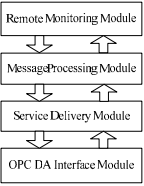
\includegraphics[scale=0.65]{XML-DA-server.png}
	\end{center}
	\begin{center}
	\textit{Fig.3 OPC XML-DA server structure.}
	\end{center}
	Remote monitoring module is used for network communication and message serialization. When receiving a request, it will create a new thread to deal with this connection request and the main thread will immediately return to monitor the next connection request. The new thread will call the HTTP message module to parse the HTTP POST request, check out the SOAP message body and give it to the message processing module. Then this thread uses SOAP as an envelope to pass the result which is returned by the message processing module to the client using HTTP.\newline
	The message processing module is used for parsing the message sent by the client to SOAP, creates a request object which is defined in the OPC XML-DA schema and passes it to the service delivery module. Then it waits for a response from the service delivery module and uses XML format as an envelope for passing the message to the remote monitoring module.\newline
	The service delivery module includes eight services defined in the OPC XML-DA specification. These services include: Get status, Read, Write, Subscribe, SubscriptionPolledRefresh, SubscriptionCancel, Browse and GetProperties. Each specific service has a request and response parameter. This service will call the appropriate function in the OPC DA interface module and then the response object will be created and returned to the message processing module.\newline
	The OPC DA intertface contains the functions of the server, data management and internal services. 
	\subsubsection{OPC security}
	The assumption that OPC XML-DA makes is that the transport will handle security. In the past, many companies have chosen to adopt a \textit{wide-open} security policy for OPC servers and have relied on firewalls to protect from intruders. When web services came to play, process control information was no longer restricted to LAN, because web services are frequently deployed outside the firewall and potentially exposing important information to everyone who has access to the Internet. \newline
	Unrestricted read access to the data is not a big problem but write access must be restricted because some intruder might write incorrect data which can cause different problems. Therefor it is recommended that vendors provide a means to globally disable the server's \textit{write} access and put it to \textit{read-only} mode.\newline
	The OPC security specifications consists of a set of conditions regarding how to secure OPC server applications, OPC client applications and any other vendor-specific security objects implemented by the OPC server. The vendor-specific security objects are server interfaces, methods and individual or set of data items. Each security object has an associated reference monitor which provides authentication for the clients to access that object. OPC security specification deals with two reference monitors for secured objects, namely:
	\begin{description}
	\item[$\bullet$]
	Windows NT reference monitor: controls access to DCOM server and clients. It validates the credentials of the clients requesting to connect to the DCOM servers and only after successful validation it provides authorization to connect.
	\item[$\bullet$]
	OPC server: is implemented to validate the credentials of the client and make the decision of providing access to its secured objects. The OPC server implements on of these levels of security: \newline
	1. Disabled security: no security is enforced. The server starts and every client can connect to it and access its data.\newline
	2. DCOM security: the access to the OPC server is controlled by the Windows NT DCOM security.\newline
	3. OPC security: the server serves as the reference monitor to control access to its secured objects.
	\end{description}
	
 \subsection{Wind farm power infrastructure}
  A wind farm is not just a collection of unrelated individual turbines. Rather, wind farms have their own system of electrical distribution, with connections to all turbines on the farm. Wind farm incorporate many components to ensure the safe, efficient and reliable generation, transmission and injection of electricity into the power grid. From the perspective of functionality and security, a wind farm can be envisioned as having two interconnected, cooperative infrastructures. The IEC international standard defined uniform design, operation and communications requirements for wind turbine suppliers.

\end{multicols}
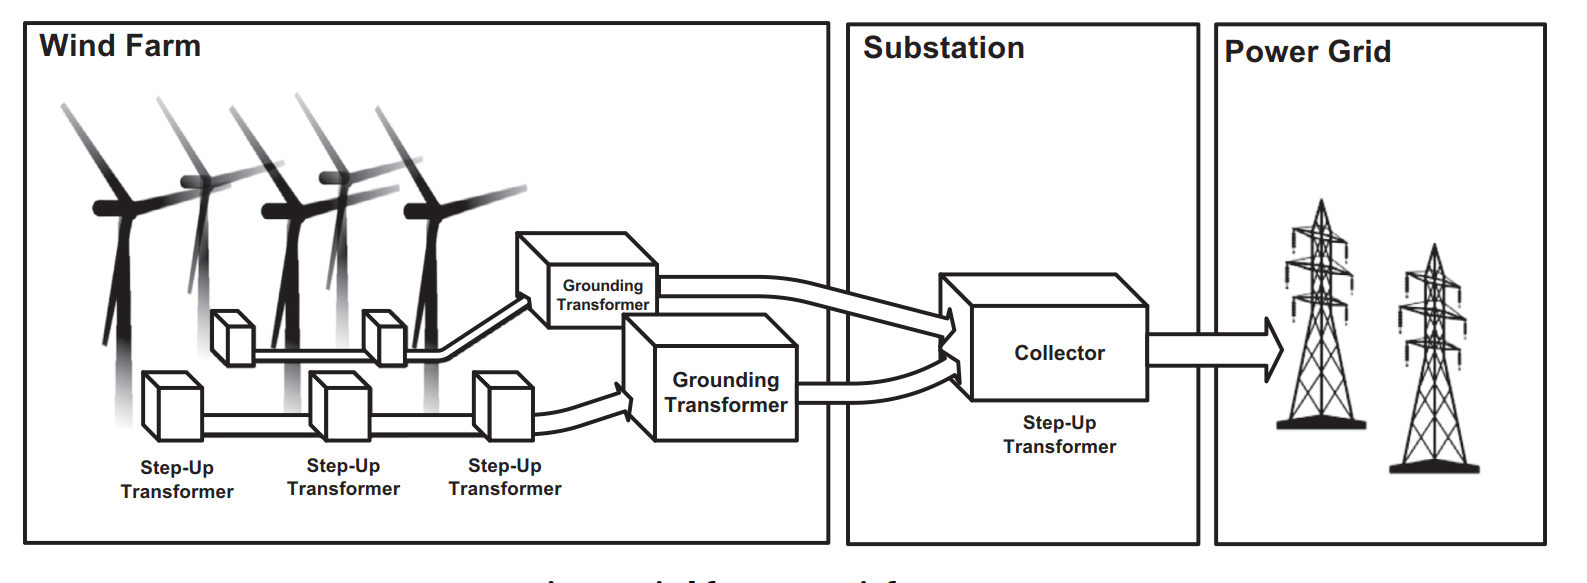
\includegraphics[scale =0.45]{windfarm_infra}
\begin{center}
	\textit{Fig.4 Wind farm power infrastructure.}
\end{center}

\begin{multicols}{2}

Figure 4 presents a schematic diagram of a wind farm power infrastructure. Wind turbines in a wind farm convert rotational kinetic energy into electricity. \newline
The electrical collections system for the entire wind farm operates at a high voltage. The voltages for the entire farm are higher than the voltage at the individual turbine generators. The purpose of the higher voltage is to decrease resistive losses. As the wind-generated electricity travels to the grid, there is a loss of electricity due to resistance. The higher voltage compensates for the resistance loss. Additionally, the farm and the various turbines are equipped with a switch.
 \subsubsection{Control, Monitoring and Data collection}
 Supervisory control and data acquisition (SCADA) system control individual turbines while also displaying and reporting information on overall wind farm operation. The wind farm operator can choose to display information about any combination of operating factors.\newline
 The wind farm operator can display information about the whole wind farm. For example, maybe there is a group of turbines that need attention, due to a wind or ground situation in a specific area of the farm.in that case, the operator can see a group of turbines and look for common readings. Or, the wind farm operator can single out one individual turbine to provide data to a wind energy technician working at that location. Any number of combinations can be displayed. The information displayed by the SCADA generally includes the following: Turbine operating states, Power level, Total energy production.
 \paragraph{DNP3 (Distributed Network Protocol)}
 DNP3 is a set of communications protocols used between components in process automation systems. Its main use is in utilities such as electric and water companies. Usage in other industries is not common. It was developed for communications between several types of data acquisition and control equipment. It plays a crucial role in SCADA systems, where it is used by SCADA Master Stations (a.k.a. Control Centers), Remote Terminal Units (RTUs), and Intelligent Electronic Devices (IEDs). It is primarily used for communications between a master station and RTUs or IEDs. ICCP, the Inter-Control Center Communications Protocol (a part of IEC 60870-6), is used for inter-master station communications. Competing standards include the older Modbus protocol and the newer IEC 61850 protocol.
 
  \subsubsection{Substations}
 Almost in every wind farm a step-up substation is built to collect all the energy generated by the turbines and received through the MV cables. The exceptions are new wind farms or existing wind farms extensions built near a substation that can be upgraded to absorb the additional energy produced: in these cases, only a control center with the SCADA and the medium voltage system is realized.
 Although there are different possible technical solutions, normally a substation will be composed by the following elements:
 \begin{description}
 	\item[$\bullet$]
 	Medium voltage system
 	\item[$\bullet$]
 	High voltage system
 	\item[$\bullet$]
 	Capacitors banks
 	\item[$\bullet$]
 	Auxiliary services
 	\item[$\bullet$]
 	Control, protection and metering system
 	\item[$\bullet$]
 	Communication system
 	\item[$\bullet$]
 	Fire protection and intruders protection systems
 \end{description}
 Substations collect the power generated by wind turbines and step up the voltage for injection into grid. Substations also serve as command and control centers. Depending on the energy output of a wind farm, there may be multiple substations.
 The operations side of a substation incorporates information technology, networking, safety and backup systems, and heating, ventilation and air conditioning (HVAC) systems. The transmissions side is air-gapped from the operations side. Unlike wind turbines, transmission control facilities have strong physical security mechanisms, including locks, cameras, motion sensors, remote alerting systems reinforced construction and fences.
 
 \subsubsection{Control Center}
 The control center provides the centralized command and control of the wind farm networks. In many cases, the center is collocated with corporate offices. Some large wind farms may have multiple control centers each responsible for a geographic region.
 The control center is typically located in a metropolitan area, although smaller control centers may be located in non-urban areas closer to the wind farms. The control center is considered to be a high-impact asset and is, therefore required to be NERC-CIP compliant according to the U.S regulations. Therefore, it implements strong physical information technology security control mechanisms. Each control center has a backup facility that can ensure continuity of operations. This paper doesn’t not consider the threats that originate from or target a control center.
     
\section{Chapter 3 : Risk Management and Ransom } 
\subsection{Introduction}
An attacker intending to disrupt wind farm operations or damage equipment would concentrate on six types of targets: (i) control networks; (ii) programmable logic/automation controllers; (iii) network devices; (iv) operator stations; (v) engineering workstations; and (vi) historians. The targets may be accessed using several alternatives. The main reason is often the money. Most often we use a ransomware with a cryptocurrency. The most famous cryptocurrency is Bitcoin. Companies can protect their systems but unfortunately full security can never be achieved.

\subsection{Definition of Risk Management}
A security risk assessment is an important element in the overall security risk
management process. Security risk management involves the process of ensuring
that the risk posture of an organization is within acceptable bounds as defined by
senior management. Each security breach has a mitigation. Th main issue in network security is that we don't know how an attacker will try to invade our system. That's why a security risk assessment allows company to simulate or imagine several kind of attacks and see if their system has a failure.\newline
There are four stages of the security risk management process:
(i) security risk assessment; (ii) test and review; (iii) security risk mitigation; and (iv) operational security.
\begin{itemize}
    \item \textbf{Security Risk Assessment} : This is an objective analysis of the effectiveness of the current security controls that protects an organization’s assets and a
    determination of the probability of losses to those assets. A security risk
    assessment reviews the threat environment of the organization, the value of
    assets, the criticality of systems, the vulnerabilities of the security controls,
    the impact of expected losses, and recommendations for additional controls
    to reduce risk to an acceptable level. Based on this information the senior
    management of the organization can determine if additional security
    controls are required.
    \item \textbf{Test and Review} : Security testing is the examination of the security
    controls against the security requirements. Security controls are determined
    during the security risk assessment and tested during security testing efforts.
    Security testing is performed more frequently than security risk assessments.
    \item \textbf{Risk Mitigation} : Risks to an organization’s assets are reduced through
    the implementation of new security controls or the improvement of existing
    controls. Security risk assessments provides information to allow the
    senior management to make risk-based decisions for the development of
    new controls or expenditure of resources on security improvements on existing controls. Security test and review efforts provide information on
    how to keep existing controls up to date. Risk can be mitigated through
    corrections and additional controls or accepted or transferred.
    \item \textbf{Operational Security} : The implementation and operation of most
    security controls are performed by operational personnel. Daily and weekly
    activities such as applying patches, performing account maintenance, and
    providing security awareness training are essential for maintaining an
    adequate security posture.
\end{itemize}

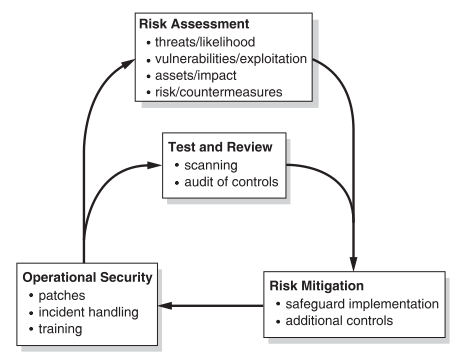
\includegraphics[scale=0.65]{security_management}
\begin{center}
	\textit{Fig.6 The role of the security risk assessment. Security risk assessments play a critical role in the security management process, providing information on the threats, assets, and risks to an organization.}
\end{center}
 
\subsection{Ransomware and cryptocurrency}
\subsubsection{Ransomware}
Ransomware is a type of malicious software from cryptovirology that threatens to publish the victim's data or perpetually block access to it unless a ransom is paid. While some simple ransomware may lock the system in a way which is not difficult for a knowledgeable person to reverse, more advanced malware uses a technique called cryptoviral extortion, in which it encrypts the victim's files, making them inaccessible, and demands a ransom payment to decrypt them.\newline
There are two main forms of ransomware in circulation today:
\begin{itemize}
    \item Locker ransomware(computer locker):
Denies access to the
computer or device
\item Crypto ransomware
(data locker): Prevents
access to files or data.
\end{itemize}
Crypto ransomware doesn’t necessarily have to use encryption to stop users from accessing their data, but the vast majority of it does. Both types of ransomware are aimed squarely at our digital lifestyle. They are designed to deny us access something we want or need and offer to return what is rightfully ours on payment of a ransom. Despite having similar objectives, the approaches taken by each type of ransomware are quite different.
In our case, the objective is to take control and stop the operation of Windfarm. The attacker would then send a email to demand money via a cryptocurrency like Bitcoin.

\subsubsection{cryptocurrency : Bitcoin}

Bitcoin is a collection of concepts and technologies that form the basis of a digital money ecosystem. Units of currency called bitcoins are used to store and transmit value among participants in the bitcoin network. Bitcoin users communicate with each other using the bitcoin protocol primarily via the Internet, although other transport networks can also be used. The bitcoin protocol stack, available as open source software, can be run on a wide range of computing devices, including laptops and smartphones, making the technology easily accessible. \newline
Users can transfer bitcoins over the network to do just about anything that can be done with conventional currencies, including buy and sell goods, send money to people or organizations, or extend credit. Bitcoins can be purchased, sold, and exchanged for other currencies at specialized currency exchanges. Bitcoin in a sense is the perfect form of money for the Internet because it is fast, secure, and borderless.\newline
\newline
Unlike traditional currencies, bitcoins are entirely virtual. There are no physical coins or even digital coins per se. The coins are implied in transactions that transfer value from sender to recipient. Users of bitcoin own keys that allow them to prove ownership of transactions in the bitcoin network, unlocking the value to spend it and transfer it to a new recipient. Those keys are often stored in a digital wallet on each user’s computer. Possession of the key that unlocks a transaction is the only prerequisite to spending bitcoins, putting the control entirely in the hands of each user.\newline
The bitcoin system, unlike traditional banking and payment systems, is based on de-centralized trust. Instead of a central trusted authority, in bitcoin, trust is achieved as an emergent property from the interactions of different participants in the bitcoin system. The transaction is flowing on per-to-per network and everything happens anonymously, hence that's the reason it is used.
 
\section{Chapter 4 : Security Breach}

\subsection{Introduction}
 According to Staggs, a Ph.D. from University of Tulsa in Tulsa in Oklahoma, there are some vulnerabilities in wind farm nowadays. He listed some overviews of vulnerabilities facing wind farms:
 \begin{itemize}
     \item Programmable automation controllers (PACs) running legacy operating systems, everything is operating as a root, use of insecure remote management services, easy to figure out default passwords, and no code signing
    \item	No authentication or encryption of control messages
    \item	No network segmentation between wind turbines
    \item	No physical security
 \end{itemize}
 Let's talk about some specific attack in the following chapter. The first thing an attacker must do is to enter in the network of Windfarm. Network devices have an IP but they don't have an online connection. They always have a private IP. They can't go to the outside and the outside can't communicate with the device. That's why an attacker must enter into the internal network. For that he has many possibilities. Once the attacker enters into the network, he can choose several targets. Each target has a specific role in the network structure. According to what he wants to do, the target, the methods and the dommage can be different in each case.
 
 
\subsection{Network Access}
Five distinct attack vectors are available to target a wind farm control network: cyber access using a wind farm vendor network; cyber access using technician equipment; and cyber via a compromised supply chain, and the most important part in our topic; physical access at a wind turbine, physical access at a substation.
 \subsubsection{Physical access at a wind turbine}
 Wind turbines are generally erected in remote locations with adequate wind speed duration. However, the physical security mechanisms that protect against unauthorized entry inside a wind turbine are fairly simplistic. Typically, the door to a turbine is secured by padlock that can be easily picked or bypassed using bolt cutters. Even if a turbine door has an expensive security mechanism that alert a control center about unauthorized entry, because of the remote location, it may take considerable time for responder to reach the turbine to investigate the unauthorized entry.
 \newline
Once inside the turbine, an attacker could access the wind farm control network by plugging a malicious device such as a Raspberry Pi or a Gustix into network switch. One option is to keep the network configuration intact and insert the malicious device as an additional node in the network. The attacker can use the malicious node to target other nodes in the network. These nodes include other connected turbines and substations. A malicious device configured as a new node in the wind farm control network is susceptible to discovery upon visual inspection as well as over the network. therefore, a more sophisticated access strategy is to position the malicious deice in a man-in-the middle configuration. This involves unplugging a network connection to a trusted device, inserting the malicious device before the device and quickly restoring network connectivity. Implanting the malicious device would cause a temporary disruption, which might be noticed at the transient nature of disruption and timely resumption of network connectivity, it is unlikely that security personnel would immediately trail to the site to investigate the anomaly. A more sophisticated approach is to hide a man-in-the-middle rouge device inside a trusted industrial control system component. This parasitic device drawn power from the same source as the control system component and would be difficult to discover without a detailed inspection involving the removal and disassembly of the control system component. Having gained access to wind farm control network, the attacker could target a variety of information technology and control system assets directly or the attacker could implant malware. The threats include obtaining information about devices, protocols, network configurations and operations; disrupting wind farm operations; and even damaging key physical component, including the wind turbine itself.
 \subsubsection{Physical access at a substation}
 Unlike wind turbines, substations have strong physical security mechanisms such as locks, cameras, motion sensors, remote alerting systems, reinforced constructions and fences. However, substations are still vulnerable to physical penetration and can also be accessed by malicious insiders. Since many substations are located in remote areas and are usually unnamed, it may take some time for security personnel to respond to the site of a breach. Having breached a substation, an attacker can apply the same techniques and tools used to gain access to the wind farm control networks; install persistent, hard-to-discover, parasitic devices; implant malware to surveil and disrupt wind farm operations; and possibly damage or destroy wind farm assets. In fact, unauthorized access to a substation could have more serious implications than a wind turbine breach. This is because the attacker can potentially manipulate the operations controls system as well as the transmission control system.
 \subsubsection{Cyber asses using technician equipment}
 Compromising operator and or service personnel equipment either directly via a flash drive or hands-on access, or indirectly via spear phishing can bridge air-gapped networks. The initial additional tools or malware (for privilege escalation, enhanced access and persistence) to eventually launch attacks against wind turbines and substations. Technicians equipment that could be compromised includes standard laptops, workstations and mobile communications devices. Of a particular interest to attackers are handled devices used by wind farm personnel to performs maintenance on turbine controls systems. This device communicates with a wind turbine control system over a common network medium (RS-232 or ethernet). Compromising such device enables an attacker to target trusted control network assets as well as physical equipment.
 \subsubsection{Cyber access via a compromised supply chain}
 This attack vector can be used to achieved similar access and effects as cyber access using technician equipment. However, in this case, information technology and industrial controls system hardware, firmware and software are compromised in the supply chain, before they are installed at a wind farm
 \newline We can’t talk about the windfarm physical attack without speaking about how to avoid the in another’s words physical security.
 
 \subsubsection{Cyber access using a wind farm vendor network}
 In many cases, wind farm vendors have unfettered remote virtual private network (VPN) access to wind farm control networks for monitoring, software upgrades and maintenance. This access may also be provided to vendors for research and development efforts, especially for evaluating product enhancements. Granting remote access to a wind farm vendor introduces risk and creates disturbing cyber attack environment. This is because the vendor network becomes a single point of access to multiple wind farm deployments, including wind farms belonging to other companies that rely on the vendors for products and services. An attacker could gain access to a vendor network in any number of ways, including via spear phishing campaigns, malicious insiders or physical breaches. After the vendors network is compromised, the attacker can leverage trust relationships to orchestrate attacks on multiple wind farms and their assets. During a security assessment of a wind farm conducted by authors of this paper, a vendor was observed to have remote access (from abroad) to the wind farm operations network. Standard network management protocols were utilized by the vendor, presumably for pushing software upgrades and performing diagnostics. Although the remote vendor communications were encrypted and tunneled over a VPN, the encapsulating protocols were outdated and unencrypted. This could enable a malicious entity to intercept, manipulate and fabricate messages, and launch a slew of attacks against wind turbines, substations and even win farm vendor networks.
 
\end{multicols}
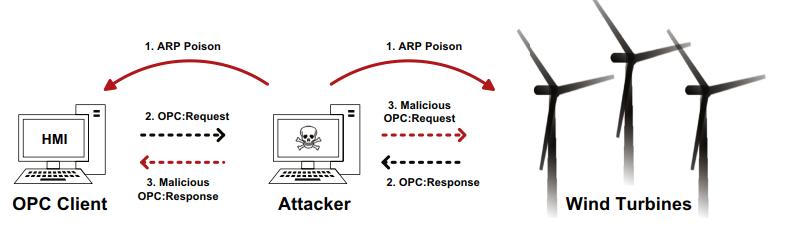
\includegraphics{cache_poison}
\begin{center}
	\textit{Fig.7 The concept of Windpoison}
\end{center}
\begin{multicols}{2}
\subsection{Network breach}

\subsubsection{WindPoison}
The Windpoison’s concept is to intercept all communication between the wind farm and the controller. They use the ARP Cache poisonning attack. The Address Resolution Protocol (ARP) is a communications protocol used for discovering the MAC address associated with a given IPv4 address. It is a critical function in Internet Protocol (IP) computer networks because based on these addresses we can determine who is the receiver of the message.
 \newline Since ARP replies are not authenticated, an attacker can send an ARP reply containing a malicious <IP, MAC> association to any host on the network thus poisoning the ARP cache of that host. The attacker may supply her MAC address in the sent malicious association which enables her to receive all the packets sent by that host to the IP address specified in the association. This way the attacker may receive all the frames originally directed to some other host. If also the cache of the real destination host is poisoned, both communication flows are under the attacker's control. \newline
In this situation, the attacker could launch a man-in-the middle. A man-in-the-middle attack (MITM) is an attack where the attacker secretly relays and changes the content of the message between wind turbine and the OPC client. When an OPC client sends a request, a falsified answer is responding to the OPC client and a wrong request is being sent to the wind turbine.  They believe they are directly communicating with each other but in fact the attacker has gained the control of the system. 


\subsubsection{WindShark}
Another way to gain control over a wind turbine is to inject some malicious request at the right time in the right place. First of all we need a tool to fabricate OPC control messages that are normally issued by an operator station in a wind farm. Then the goal is to replay these OPC request to the wind turbine. Since the message comes from the attacker, he can do whatever he wants. It's the concept of the WindShark. With Windshark, we can demonstrate the ease with which the operation of a wind turbine could be manipulated by a malicious entity. Windshark transmits OPC-XML-DA write request messages to the target turbine at the right time to gain the control of the wind turbine. That is when the write access is obtained. \newline
A typical use case involves Windshark being installed in a rogue device that is connected to the operations control system. After performing network controls to identify an accessible wind turbine, the attacker can start executing his malicious request. A more sophisticated technique involves the use of the computer worm concept to maliciously control a wind turbine.The idea is to load a malicious program and this program could modify the control logic, change process control variables and setpoints, and issue unauthorized control commands to slave programmable logic controllers in the nacelle or rotor. The computer worm could also be designed to propagate to programmable automation controllers in other wind turbines, potentially impacting an entire wind farm.


\includegraphics[scale=0.5]{Windshark}
\begin{center}
	\textit{Fig.8 The concept of Windshark}
\end{center}

	
\subsection{Mitigation}

\subsubsection{Internal firewall}
The flat logical design of the operations control network and inadequate or non-existent network access controls were leveraged in all the attack scenarios described above. An improvement solution is to isolate turbines, especially since there appears to be no operational requirement for turbine-to-turbine communications. And we can avoid contaminating  others wind turbine if one turbine is getting caught by an attacker. Wind turbine isolation can be implemented in the operations control network by retrofitting an internal firewall and they can add/create a tunnel at each turbine. This way broadcasting is avoided and the wind turbine receives the messages it was supposed to receive.
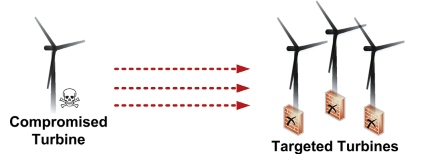
\includegraphics[scale=0.8]{internalfirewall}
\begin{center}
	\textit{Fig.9 The concept of internal firewall}
\end{center}
The first isolation solution is to use inline firewalls with strict IP-based rule sets that prevent inter-turbine communications by default. A whitelist rules set can be better if the IP of each device doesn't change. A whitelist is a list or a register of entities that provides a particular privilege, service, access or recognition. Entities on the list will be approved and all the others will be rejected. Whitelisting is better then blacklisting because we can't list all vulnerabilities and new security breaches are being discovered everyday.
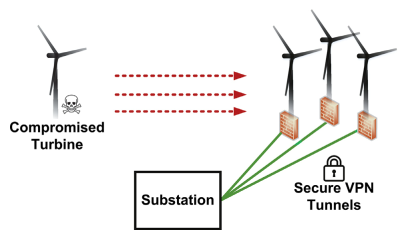
\includegraphics[scale=0.85]{vpn}
\begin{center}
	\textit{Fig.10 The concept of VPN tunnels}
\end{center}
A more sophisticated and secure strategy for isolating turbines is to implement a “bump-in-the-wire” solution that provides end-to-end encryption for each turbine. This solution, which is presented in Fig. 11 , involves a dedicated VPN connection from each turbine to a substation (using a public key infrastructure with a unique key pair 
for each turbine). This tunnels all operations control network communications over encrypted links. Unless the VPN server or key management process is compromised, an attacker would be unable to communicate with a turbine control system. 


\subsubsection{Message encryption}
In several cases, insecure OPC server implementations were identified during the security assessments of wind farms conducted by the authors of this paper (e.g., no encryption or authentication). In many instances, OPC-XML-DA was used to poll and set wind turbine data and control parameters from remote operator stations. The implementation of such a web-based protocol should adhere to the guidance provided by IEC 61400-25; for example, the protocol should be implemented over SSL/TLS in order to combat the attacks described in this paper.
\newline Transport Layer Security (TLS).- and its predecessor, Secure Sockets Layer (SSL), are cryptographic protocols that provide communications security over a computer network. The Transport Layer Security protocol aims primarily to provide privacy and data integrity between two communicating computer applications.The TLS connections have one or more of the following properties:
\begin{itemize}
	\item The connection is private (or secure) because symmetric cryptography is used to encrypt the data transmitted. The keys for this symmetric encryption are generated uniquely for each connection and are based on a shared secret negotiated at the start of the session. The server and client negotiate the details of which encryption algorithm and cryptographic keys to use before the first byte of data is transmitted. The negotiation of a shared secret is both secure and reliable.
	\item The identity of the communicating parties can be authenticated using public-key cryptography. This authentication can be made optional, but is generally required for at least one of the parties .
	\item The connection ensures integrity because each message transmitted includes a message integrity check using a message authentication code to prevent undetected loss or alteration of the data during transmission
\end{itemize}

\subsection{Physical security} 
Perhaps the most significant threat to wind farm is physical access to wind turbines and substations that enables an attacker to target the operations and transmission control networks. As mentioned above, existing physical security mechanisms are relatively weak, and the turbines and substations are typically sanctioned at remote locations. Efforts should be made to outfit every turbine with strong locking mechanisms with multifactor authentication, motion sensors, security cameras and remote alarm notifications system. Additionally, management should assign security personnel who are always ready to respond in a timely manner. Substations are very important components of a wind farm physical breaches of substations can be leveraged to wreak havoc on electricity generation and transmission assets. In addition to locking mechanisms, motion sensors, security cameras and remote alarms, substations should be fortified to the extent possible to defeat breaches of doors, windows, walls and roofs

\section{Chapter 5 : Conclusion }
The focus on renewable energy has significantly increased the number of wind farm deployments in countries around the world. Nowadays, in the wind farm infrastructure, there are a lot of security breaches and insecure protocols are used. That will expose wind farms to myriad threats. Although the threat may be known and there might be existing solutions against that particular threat, the problem arises when companies use common across wind farm configurations and vendor products and this leads to a risk which causes all the incidents in the wind farm.

%\subsection{Introduction}
% \textbf{Talk about the risk which we can prevent}
% \lipsum[1]




%\subsection{Physical Access}
%derpde
% \subsubsection{Access Control}
% \lipsum[1]

 %\subsubsection{Locking System}
 %Und noch etwas Text... \cite{muster} \newline
 %\lipsum[1]
 %\subsubsection{Quick Response}
 %\lipsum[1]

 
%\subsection{Network Mitigation}
% \subsubsection{SSL/TLS}
% \lipsum[1]
% \subsubsection{VPN}
% \lipsum[1]
% \subsubsection{Access restriction}
% \textbf{White List}
% \lipsum[1]
 
%\subsection{Best Practice}
% \lipsum[2]
\end{multicols}
\newpage

\bibliographystyle{lit}
\bibliography{lit}
\begin{itemize}
\item Wind Energy Engineering, by Trevor M. Letcher.
\item Wind Power Generation by Paul Breeze. 
\item Understanding Wind Power Technology: Theory, Deployment and Optimisation by Alois Schaffarczyk. 
\item http://ieeexplore.ieee.org/stamp/stamp.jsp?arnumber=4558422 
\item https://link.springer.com/chapter/10.1007/978-1-4302-1955-2\_14e
\item http://ieeexplore.ieee.org/stamp/stamp.jsp?arnumber=4020022\&tag=1 
\item https://ac.els-cdn.com/S1876610212002500/1-s2.0-S1876610212002500-main.pdf?\_tid=c1dc34d2-e41e-11e7-a91c-00000aab0f6b\&acdnat=1513620821\_4aab5851aa74825cdd849f19da59dcbf 
\item Industrial Process Automation Systems by Y. Jaganmohan Reddy, B.R. Mehta
\item http://www.diit.unict.it/users/scava/dispense/II/OPCDataAccessXMLSpecification.pdf
\item Renewable Energy: Selected Issues Volume I, Volume 1
edited by Manuel Pérez-Donsión, Silvano Vergura, Gianpaolo Vitale

\end{itemize}
\end{document}



